\chapter{CHỌN THÂN MÁY, BULÔNG VÀ CÁC CHI TIẾT KHÁC}
    \section{TÍNH TOÁN VỎ HỘP}
        \begin{longtable}{|p{7.5cm}|p{8.3cm}|}
            \hline
            \textbf{Tên gọi} & \textbf{Biểu thức tính toán} \\
            \hline
            Chiều dày: & \\
            - Thân hộp, $\delta$ & $\delta = 10$ (mm) \\
            - Nắp hộp, $\delta_1$ & $\delta_1 = 8$ (mm) \\
            \hline
            Gân tăng cứng: & \\
            - Chiều dày, $e$ & $e = 10$ (mm) \\
            - Chiều cao, $h$ & $h = 103$ (mm) \\
            - Độ dốc & $6:1$ \\
            \hline
            Đường kính: & \\
            - Bu lông nền, $d_1$ & $d_1 > 0.04a + 10 > 12, d_1 = 16$ (mm) \\
            - Bu lông cạnh ổ, $d_2$ & $d_2 = (0.7 \div 0.8)d_1 = 14$ (mm) \\
            - Bu lông ghép bích nắp và thân, $d_3$ & $d_3 = (0.8 \div 0.9)d_2 = 10$ (mm) \\
            - Vít ghép nắp ổ, $d_4$ & $d_4 = (0.6 \div 0.7)d_2 = 10$ (mm) \\
            - Vít ghép nắp cửa thăm dò, $d_5$ & $d_5 = (0.5 \div 0.6)d_2 = 6$ (mm) \\
            \hline
            Mặt bích ghép nắp và thân: & \\
            - Chiều dày bích thân hộp, $s_1$ & $s_1 = (1.4 \div 1.8)d_3 = 18$ (mm) \\
            - Chiều dày bích nắp hộp, $s_2$ & $s_2 = (0.9 \div 1)s_3 = 15$ (mm) \\
            - Bề rộng bích nắp và thân, $S_1$ & $S_1 = 43$ (mm) \\
            - Bề rộng mặt bích ổ đỡ, $S_2$ & $S_2 = 52$ (mm) \\
            - Bề rộng mặt đế hộp, $S_3$ & $S_3 = 60$ (mm) \\
            \hline
            Kích thước gối trục: & \\
            - Khoảng cách từ tâm bu lông $d_2$ đến thành trong ổ: $C$ & $C = 37$ (mm) \\
            - Bề rộng mặt ghép bu lông cạnh ổ, $K$ & $K = 50$ (mm) \\
            - Chiều cao h. & Phụ thuộc tâm lỗ bu lông và kích thước mặt tựa. \\
            \hline
            \pagebreak    
            \hline
            Khe hở giữa các chi tiết & \\
            - Giữa bánh răng với thành trong hộp & $\Delta \geq (1 \div 1,2)\delta = 10$ (mm) \\
            - Giữa đỉnh bánh răng lớn với đáy hộp & $\Delta_1 \geq (3 \div 5)\delta = 30$ (mm) \\
            \hline
            Số lượng bu lông nền, $Z$ & $Z = \frac{L + B}{200 \div 300} = 3$ \\
            & $L$: chiều dài hộp 396 mm \\
            & $B$: chiều rộng hộp 188 mm \\
            \hline
            \caption{Các thông số tính toán vỏ hộp}
        \end{longtable}
    \section{CÁC CHI TIẾT KHÁC}
        \subsection{Vít vòng}
            \begin{figure}[H]
                \centering
                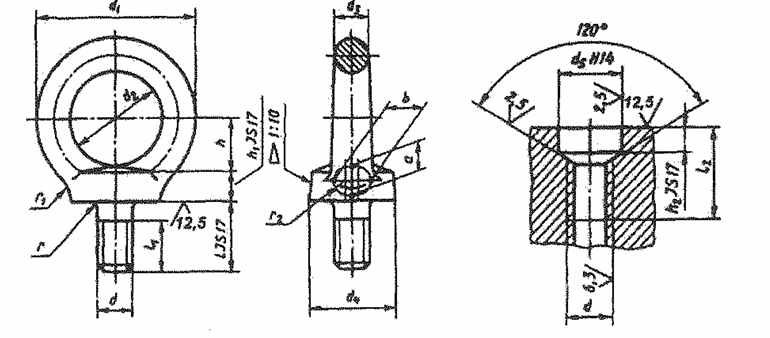
\includegraphics[width=0.8\textwidth]{pictures/ring_screw.png}
                \caption{Vít vòng}
                \label{ring_screw}
            \end{figure}
            \hspace*{0.6cm}Để nâng và vận chuyển hộp giảm tốc trên nắp và thân thường ngoài bu lông ta sử dụng vòng móc. \\
            \hspace*{0.6cm}Do đây hộp giảm tốc bánh răng trụ 1 cấp và khoảng cách trục $a = 160$ mm. Từ bảng 10.7, tài liệu tham khảo \cite{tkmctm} $\rightarrow$ Trọng lượng hộp giảm tốc $Q = 80$ (kg). \\
            \hspace*{0.6cm}Từ bảng 10.6, tài liệu tham khảo \cite{tkmctm}, ta chọn vít vòng M8 với các thông số: 
            \begin{longtable}{|c|c|}
                \hline
                \textbf{Thông số} & \textbf{Giá trị (mm)} \\
                \hline
                Đường kính vít vòng $d$ & 8 \\
                \hline
                Đường kính vòng ngoài, $d_1$ & 36 \\
                \hline
                Đường kính vòng trong, $d_2$ & 20 \\
                \hline
                $d_3$ & 8 \\  
                \hline
                $d_4$ & 20 \\
                \hline
                $b$ & 10 \\
                \hline
                $h$ & 12 \\
                \hline
                $h_1$ & 6 \\
                \hline
                $l$ & 18 \\
                \hline
                $l_1$, lớn hơn & 12 \\
                \hline
                $r$ & 2 \\
                \hline
                $r_1$ & 4 \\
                \hline
                Khối lượng & 0.05 \\
                \hline
                \centering $d_5$ & 13 \\
                \hline
                $h_2$ & 5 \\
                \hline
                \centering $l_2$, lớn hơn & 19 \\
                \hline
                \caption{Thông số vít vòng}
            \end{longtable}
        \subsection{Chốt định vị}
            \hspace*{0.6cm}Đảm bảo vị trí tương đối giữa nắp và thân hộp trước và sau khi gia công cũng như khi lắp ghé, dùng 2 chốt định vị. Nhờ chốt định vị, khi siết bulông không làm biến dạng vòng ngoài của ổ (do sai lệch vị trí tương đối của nắp và thân hộp), do đó làm loại trừ một trong các nguyên nhân làm ổ chóng hỏng.\\
            \hspace*{0.6cm}Chọn chốt hình côn, có thông số như sau:
            \begin{figure}[H]
                \centering
                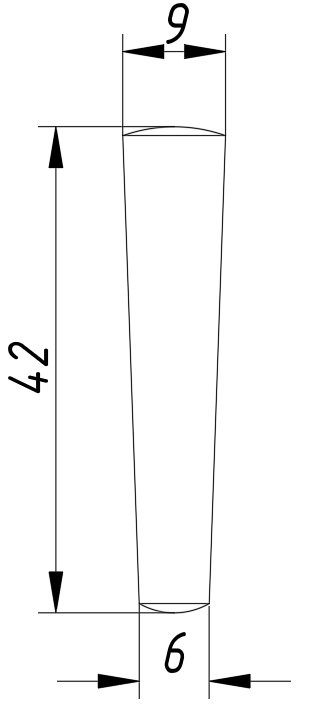
\includegraphics[width=0.2\textwidth]{pictures/position_pin.png}
                \caption{Chốt định vị}
                \label{position_pin}
            \end{figure}
            \begin{table}[H]
                \centering
                \begin{tabular}{|c|c|c|c|}
                    \hline
                    \textbf{Thông số} & $\mathbf{d_1}$ & $\mathbf{d}$ & $\mathbf{l}$ \\
                    \hline
                    \textbf{Giá trị (mm)} & 9 & 42 & 6 \\
                    \hline
                \end{tabular}     
                \caption{Thông số chốt định vị}           
            \end{table}
        \subsection{Cửa thăm}
            \begin{figure}[H]
                \centering
                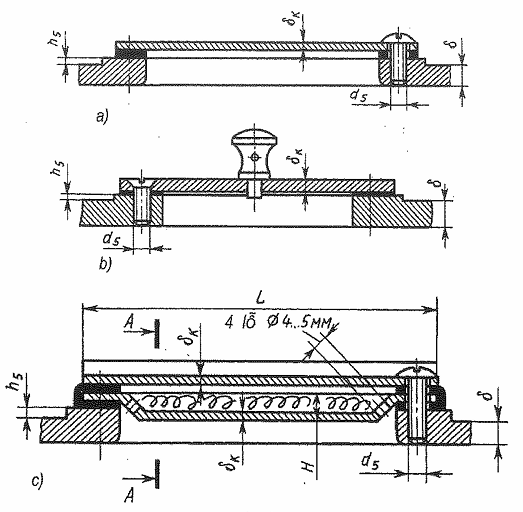
\includegraphics[width=0.6\textwidth]{pictures/oil_dipstick_cap.png}
                \caption{Nắp cửa thăm}
                \label{oil_dipstick_cap}
            \end{figure}
            \hspace*{0.6cm}Để kiểm tra, quan sát các chi tiết máy trong hộp khi lắp ghép và để đổ dầu vào hộp, trên đỉnh hộp có làm cửa thăm. Cửa thăm được đậy bằng nắp. Trên nắp có lắp thêm nút thông hơi \\
            \hspace*{0.6cm}Kích thước nắp cửa thăm dầu:
            \begin{longtable}{|c|c|c|c|c|c|c|c|c|c|}
                \hline
                \textbf{Thông số} & $\mathbf{A}$ & $\mathbf{B}$ & $\mathbf{A_1}$ & $\mathbf{B_1}$ & $\mathbf{C}$ & $\mathbf{K}$ & $\mathbf{R}$ & \textbf{Kích thước vít} & \textbf{Số vít}\\
                \hline
                \textbf{Giá trị (mm)} & 100 & 75 & 150 & 12O & 125 & 100 & 12 & M8x22 & 4 \\
                \hline
                \caption{Thông số nắp cửa thăm}
            \end{longtable}
        \subsection{Nút thông hơi}
            \hspace*{0.6cm}Khi làm việc, nhiệt độ trong hộp tăng lên. Để giảm áp suất và điều hòa không khí bên trong và ngoài hộp. Ta dùng nút thông hơi. Nút thông hơi được lắp trên nắp cửa thăm.
            \begin{figure}[H]
                \centering
                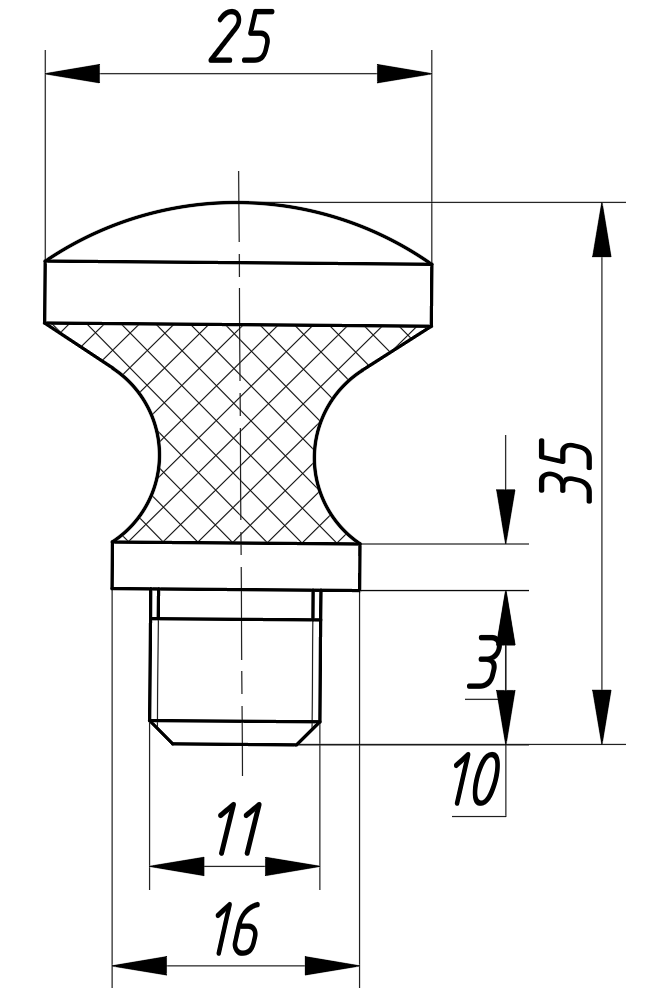
\includegraphics[width=0.3\textwidth]{pictures/ven_plug.png}
                \caption{Nút thông hơi}
                \label{ven_plug}
            \end{figure} 
            \begin{table}[H]
                \centering
                \begin{tabular}{|c|c|c|c|c|c|c|}
                    \hline
                    \textbf{Thông số} & $\mathbf{d}$ & $\mathbf{D}$ & $\mathbf{D_1}$ & $\mathbf{L}$ & $\mathbf{l}$ & $\mathbf{b}$  \\
                    \hline
                    \textbf{Giá trị (mm)} & M11x1.75 & 16 & 25 & 35 & 10 & 3 \\
                    \hline 
                \end{tabular}     
                \caption{Thông số nút thông hơi}           
            \end{table}
        \subsection{Nút tháo dầu}
            \hspace*{0.6cm}Sau một thời gian làm việc, dầu bôi trơn chứa trong hộp bị bẩn (do bụi bặm và do hạt mài) hoặc bị biến chất, do đó cần phải thay dầu mới. Để tháo dầu, ở đáy hộp có lỗ tháo dầu. Khi làm việc, lỗ được bít kín bằng nút tháo dầu. Thông số nút tháo dầu được tham khảo bảng 18-7 tài liệu tham khảo \cite{tltk2}.\\ 
            \begin{figure}[H]
                \centering
                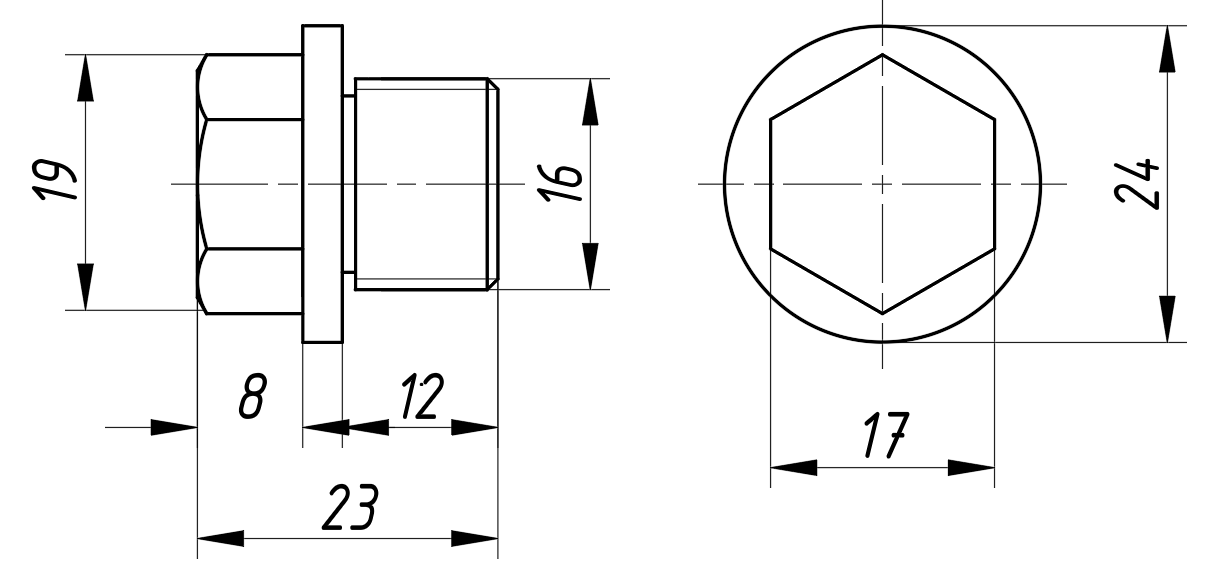
\includegraphics[width=0.7\textwidth]{pictures/oil_drain_plug.png}
                \caption{Nút tháo dầu}
                \label{oil_drain_plug}
            \end{figure}
            \begin{table}[H]
                \centering
                \begin{tabular}{|c|c|}
                    \hline
                    \textbf{Thông số} & \textbf{Giá trị (mm)} \\
                    \hline
                    $\mathbf{d}$ & M16x1.5 \\     
                    \hline
                    $\mathbf{b}$ & 12 \\
                    \hline
                    $\mathbf{m}$ & 8 \\
                    \hline
                    $\mathbf{f}$ & 3 \\
                    \hline
                    $\mathbf{L}$ & 23 \\
                    \hline
                    $\mathbf{c}$ & 2 \\
                    \hline
                    $\mathbf{q}$ & 13.8 \\
                    \hline
                    $\mathbf{D}$ & 26 \\
                    \hline
                    $\mathbf{S}$ & 17 \\
                    \hline
                    $\mathbf{D_{0}}$ & 19.6 \\
                    \hline
                \end{tabular}     
                \caption{Thông số nút tháo dầu}
            \end{table}
        \subsection{Que thăm dầu}
            \hspace*{0.6cm}Để kiểm tra mức dầu trong hộp, ta dùng que thăm dầu.\\
            \hspace*{0.6cm}Que thăm dầu có các thông số như sau:
            \begin{figure}[H]
                \centering
                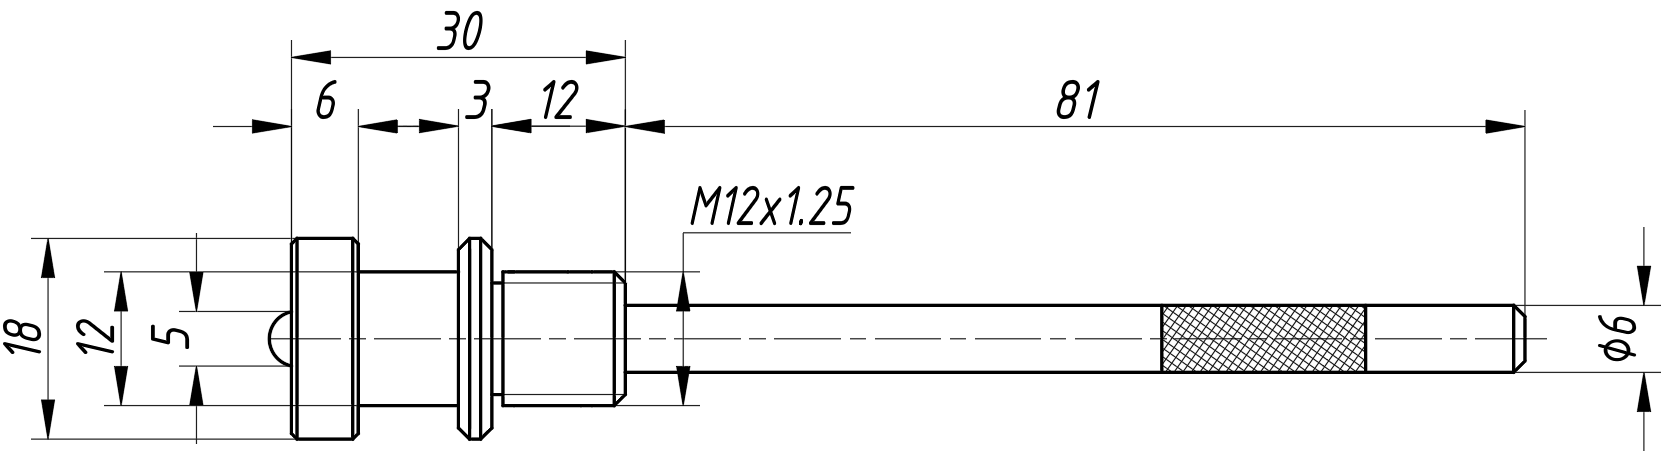
\includegraphics[width=0.7\textwidth]{pictures/oil_dipstick.png}
                \caption{Que thăm dầu}
                \label{oil_dipstick}
            \end{figure}
            \begin{table}[H]
                \centering
                \begin{tabular}{|c|c|c|c|c|c|c|c|c|c|}
                    \hline
                    \textbf{Thông số} & $\mathbf{d}$ & $\mathbf{d_1}$ & $\mathbf{d_2}$ & $\mathbf{D}$ & $\mathbf{D_1}$ & $\mathbf{L_1}$ & $\mathbf{l}$ & $\mathbf{l_1}$ & $\mathbf{b}$ \\
                    \hline
                    \textbf{Giá trị (mm)} & M12x1.25 & 5 & 6 & 18 & 12 & 30 & 12 & 6 & 3 \\
                    \hline
                \end{tabular}     
                \caption{Thông số que thăm dầu}           
            \end{table}
        \subsection{Vòng phớt}
            \hspace*{0.6cm}Vòng phớt là loại lót kín động gián tiếp nhằm mục đích bảo vệ ổ khỏi bụi bặm, chất bẩn, hạt cứng và các tạp chất khác xâm nhập vào ổ. Những chất này làm ổ chóng bị mài mòn và bị han gỉ. Ngoài ra, vòng phớt còn đề phòng dầu chảy ra ngoài. Tuổi thọ ổ lăn phụ thuộc rất nhiều vào vòng phớt. \\
            \hspace*{0.6cm}Vòng phớt được dùng khá rộng rãi do có kết cấu đơn giản, thay thế dễ dàng. Tuy nhiên có nhược điểm là chóng mòn và ma sát lớn khi bề mặt trục có độ nhám cao. 
            \begin{figure}[H]
                \centering
                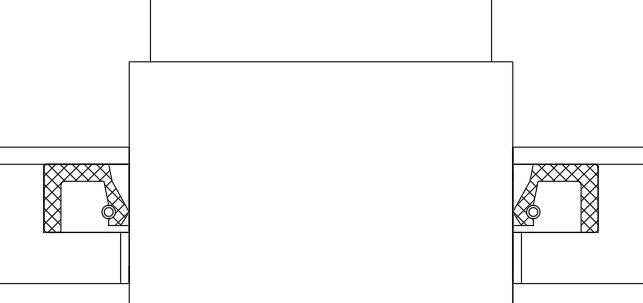
\includegraphics[width=0.5\textwidth]{pictures/seal.png}
                \caption{Vòng phớt}
                \label{seal}
            \end{figure}
        \subsection{Vòng chắn dầu}
            \hspace*{0.6cm}Vòng chắn dầu dùng để ngăn mỡ trong ổ và dầu trong hộp. Vòng gồm 3 rãnh tiết diện tam giác có góc ở đỉnh 60$^\circ$. Khoảng cách giữa các đỉnh là 3 (mm). Vòng cách mép trong thành hộp khoảng (0.5 $\div$ 1) (mm). Khe hở giữa vỏ với mặt ngoài của vòng ren là 0.43 (mm).
            \begin{figure}[H]
                \centering
                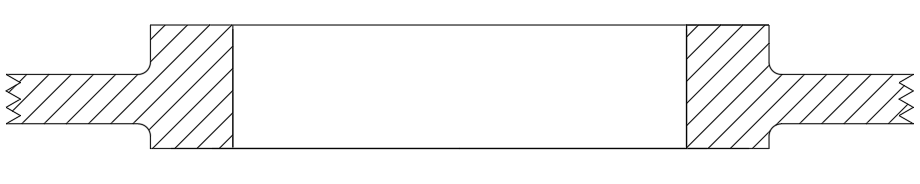
\includegraphics[width=0.5\textwidth]{pictures/oil_shield.png}
                \caption{Vòng chắn dầu}
                \label{oil_shield}
            \end{figure}
           
            